\documentclass{article}


%\usepackage{times}

\usepackage[UTF8]{ctex}
\usepackage{amsmath,amssymb,amsfonts}
\usepackage{algorithmic}
%\setlength{\marginparwidth}{0.6in}
\usepackage{diagbox}
\usepackage{graphicx}
\usepackage{textcomp}

\usepackage{booktabs} % For formal tables

\newlength{\figwidths}
\setlength{\figwidths}{3.3in}
\newlength{\expwidths}
\setlength{\expwidths}{3.6in}
\newlength{\expwidthd}
\setlength{\expwidthd}{7.2in}


% general ---------------------------------------------
\newcommand{\nop}[1]{}



\begin{document}

\title{Time Series Data Cleaning}

\maketitle


\begin{abstract}
错误在时间序列中普遍存在,例如 GPS 轨迹中存在明显的错误等等。这种情况在工业领域中尤为常见,以某风电装备数据为例,其收集的风机传感序列数据存在大量缺失值、异常值、时间标签无法对齐等错误。某地区风场每天约有 24\% (约 800 万个)数据点,31\%(约 5000 台)设备,因数据错误而无法存入数据库(入 库),造成了严重的数据资产损失。面对这些含有错误的时间序列,除了常见的保留错误数据、全部丢弃错误数据、进行人工检查之外,还可以利用两类在数据库中广泛使用的清洗算法对时间序列数据进行自动清洗,即基于平滑的清洗算法和基于模型的清洗算法…

\end{abstract}
%\begin{IEEEkeywords} data cleaning, data quality, time series. \end{IEEEkeywords} 

%-------------------------------------------------------------------------
\section{Introduction}
\subsection{研究背景与意义}
Temporal data are data that vary over time \cite{DBLP:journals/tkde/JensenS99}, also known as time series data.
Temporal data are characterized by data elements being a function of time. In general, the datum takes the following form:
$$D=\{(t_1, y_1), (t_2, y_2), \dots, (t_n, y_n)\}$$
where $t_i, 1 \leq i \leq n$ are time stamps and $y_i = f(t_i)$ are data values.时间序列在金融经济、气象水文、信号处理、 工业制造等众多领域都有着广泛的应用 [1–3] 。尤其是在金融经济领域,时间序列最主要的应用就是预测未来的商品(股票)价格走势。然而时间序列数据中错误却十分常见,即使在人们普遍认为相当准确的数据集中依然存在错误,例如雅虎财经上关于股票信息的正确率为93\%。数据中的错误、冲突以及非一致性所带来的成本和风险,已经在企业和政府部门引起广泛关注。Eckerson[5]的报告指出,具有数据质量问题的客户数据使得美国企业每年的邮资成本高达6100亿美元。除此之外,随着智能制造的逐步推广,以传感数据为代表的工业大数据持续生成,Palmer[6]指出,即便是一般的 RFID 应用每天也会产生 1G 级别的数据, 由于RFID 等设备本身的不确定性,其数据质量难以保证。上述数据质量问题在工业领域中尤为显著,
Temporal data is significant in industry, where there are all kinds of sensor devices capturing data from physical world uninterruptedly.
While the sensor devices are often unreliable and produce missed readings and unreliable readings \cite{DBLP:conf/pervasive/JefferyAFHW06}.这些质量不高的数据,对后续的数据分析等业务产生了严重影响。
As a result, temporal data are often large and dirty.
In recent work, the data quality issues in temporal data are studied, 
since they pose unique data quality challenges due to the presence of autocorrelations, trends, seasonality, and gaps in the temporal data \cite{DBLP:journals/debu/DasuDS16}.
如何改进数据质量成为一个重要的研究课题和实践内容,涉及统计、管理、计 算机科学等领域。Shilakes 等人[7]统计,数据质量的相关市场年增长率约为 17\%,远高于IT行业的 7\% 年增长率。例如,在数据仓库项目开发中,约有 30\%-80\% 的 时间和成本是用于数据清洗方面的工作。Batini 等人[8] 指出,如何有效地识别并修 复数据中的冲突和不一致性,已经成为数据管理领域一个重要的研究课题。 
时间序列中出现的错误,既可能是时间戳错误,又可能是观测值错误。对于 时间戳可能的错误,Song 等人[9] 提出了清洗时间戳的算法。而本文则重点调研了观测值错误下的现有处理方法,在后文提到时间序列中存在错误特指观测值(数值)上的错误。 
面对含有错误的时间序列,人们常用三类处理方法:一是保留错误数据。即不 对得到的时间序列进行任何处理。这样做会使得错误仍然存在于时间序列中,对 查询分析等一系列后续应用造成无法预料的后果;二是全部丢弃错误数据。即对 时间序列进行异常检测,将检测出来的异常数据丢弃;三是数据清洗。数据清洗又分为人 工清洗和自动清洗两种。毫无疑问,人工清洗会有较高的准确率,然而却因为费 时费力而难以实行。本文将对时间序列数据的异常检测算法和清洗算法做综述,通过对已有方法的总结,给对时间序列数据清洗感兴趣的学者一个参考或者指导,并基于此进一步讨论了时间序列清洗问题今后可能存在的挑战和新的研究热点。



\subsection{问题特点}
受到[10,11] 两篇文章关于时间序列错误类型划分的启发,本文将时间序列中普遍的错误情况归纳为三类,即单点大错误、单点小错误和连续错误三大类别。本文以图1.1所示的某股票连续 32 个交易日的股票价格为例,详细地描述这三类错误的特点。图中的蓝线表示该股票在这 32 个交易日的真实价格,即真实值(正确值),而黑线表示某网站爬取的该股票价格,即观测值。由于种种原因,很可能出现观测 值和真实值不一样的情况。可以看到,在第5个交易日,观测值为1,而真实值为1.25;在第15个交易日,观测值为2.5,而真实值为1.2;在第 23-26这连续四个交易日中,观测值均为 0,而真实值分别为1.2,1.1,1.2和 1.15。
\par A. 单点大错误。 所谓单点错误,即在时间序列中,错误并不连续出现,只在单个数据点上间隔发生。而大错误,指的是该数据点的观测值与真实值相差距离 较大。要注意的是,距离相差较大还是较小是相对的,和数据集的真实情况密切 相关。如图1.1中第 15 个交易日,观测值与真实值相差 1.3,相比于观测值与真实 值相差为 0.25 的第 5 个交易日,该数据点出现的误差明显很大,故该数据点的错 误类型为单点大错误。实际上,单点大错误在日常生活中十分常见,例如采用游 标记录的机动车油位数据,在路面行驶遇到颠簸时,就会出现单点大错误。 
\par B. 单点小错误。 和单点大错误类似,即错误并不连续出现,只在单个数据点 上间隔发生。只是该数据点的观测值与真实值相差距离较小。如图1.1中的第 5 个 交易日,即为单点小错误。如[12] 所言,单点小错误背后的原理是人们或者系统总 是尽量最小化可能产生的错误。例如人在抄写文件时可能仅仅有一些小的疏漏。 
\par C. 连续错误。 所谓连续错误,即在时间序列中,连续若干个时间点均出现错 误。具体而言,连续错误还可以继续细分为几个类型 [11] ,但本文不再详细区分。如 图1.1中的第 23-26 个交易日观测值均为 0,即出现了连续错误。在实际生活中连续 错误也十分常见,例如手持智能手机在路上行走时,附近的高大建筑物可能会对 采集到的 GPS 信息造成持续的影响。另外,系统的卡顿也有可能造成连续错误。 

\subsection{面临挑战 }
对于时间序列数据清洗这个问题而言,通过调研发现以下三个难点:
\par(1)数据量大,错误率高
时间序列数据主要来源为传感器采集。尤其是在工业领域,遍布于机械各处的传感器一直在对机械的运转进行着实时的监控。这些传感器采集频率往往在秒这一级别。例如某场风机传感器采集间隔为7秒,而每一时刻一台风机平均下来会记录2000个以上的工况,每天共采集数据3千万条以上,工况 600 亿以上。规模相当庞大。然而传感器采集到的数据 往往并没有那么准确,有些是因为其观测的物理量很难准确测量,例如在钢厂中,连铸坯表面温度会受到环境干扰的影响,无法准确测量;而有些可能 因为传感器自身的电量等原因,导致采集失真。传统的数据清洗方法效率较低而且准确度也不高。 
\par(2)具有持续性 
时间序列数据和关系型数据最大的不同在于时间序列具有持续性,即时间序列会源源不断地产生和存储。因此对于时间序列来讲,清洗算 法是否支持在线运算(实时运算)十分重要。在线异常检测或清洗算法能够 实时监控物理量的情况,发现问题及时报警或进行合理范围内的清洗,能够高效可靠地保证生产线的持续运转。即时间序列清洗算法不仅要求支持在线计算(或者是流式计算),而且有良好的吞吐率。 
\par(3)最小修改原则
时间序列往往含有很多错误。现今广泛使用的时间序列清 洗方法大多利用了平滑过滤 (Smoothing) 的原理,然而此种做法可能会很大程度地 改变原始数据,从而丢失了原本数据中蕴含的信息。业界认为,数据清洗需要避免改变原本正确的数据,应该依据最小修改原则,即做出的改变越小越好。

\subsection{Organization}
在接下来得内容里,第2章主要综述了基于统计的清洗算法;第3章主要综述了基于约束的清洗算法;第4章主要综述了基于模型的清洗算法;第5章主要综述了时间序列数据异常检测算法;第6章主要综述了时间序列清洗算法的工具和评价标准;第7章对本文做了总结,并讨论了与时间序列数据清洗相关的未来工作方向。



\section{基于平滑的清洗算法}
平滑技术经常被用来消除噪声数据,尤其是数值型数据。比较简单的算法有低通滤波,即过滤掉数据集中出现频率较低的,这类技术的特点是时间开销小,但是会修改原数据,会使得分析的结果失真,导致结果的不确定性,因此时间序列数据清洗的实际应用中应用的并不多,平滑算法的研究较多集中的SMA和AR和卡尔曼滤波模型和空间状态模型等算法上,因此本章将主要介绍这4种算法。
\subsection{SMA}
滑动平均系列算法 [13] 被广泛使用于时间序列进行平滑处理和时间序列预测中。一个最简单的滑动平均算法 SMA 计算最近观察到的N个数据点数值的平均值,该平均值会被用于预测接下来的时刻的数据点的数值。SMA中,过去观察到的数据点具有相等的权重。

\par 对于给定的时间序列数据y(t),为了消除数据中的错误或者噪声,可以认为数据y(t)在某个时间窗口上是平稳的,并计算局部平均;这样沿全长 N 个数据逐一小区间上进行不断的局部平均 , 

\par 即可得出较平滑的测量结果, 而滤掉噪声或者错误数据。
在滑动平均算法 WMA 中,窗口中不同位置的数据点具有不同的权重,例如将这些数据点与待预测数据点之间的时间距离的倒数作为每个数据点的权重。即距离越远的数据点,起到的作用越小。类似地,指数带权滑动平均算法 EWMA[14] 中每个数据点的权重,随着时间距离的增大权重呈指数级递 减,该算法主要用于非稳态的时间序列 [15–17] 。

\subsection{AR}

自回归模型(Autoregressive Model)是用自身做回归变量的过程,即利用前期若干时刻的随机变量的线性组合来描述以后某时刻随机变量的线性回归模型[1],它是时间序列中的一种常见形式[2]。
\par 则称时间序列y(t)为服从(p,q)阶自回归滑动平均混合模型。
差分自回归移动平均法(ARIMA)


\subsection{空间状态模型}
状态空间模型假设所研究的系统随时间的变化可由一个不可观测向量序列所确定,通常与该序列相伴的是一个可观测序列,两者的关系由状态空间模型来判别。状态空间一般由状态方程和观测方程构成,状态方程表示从目前状态向下一个时刻状态的转换方法,即状态间的转换关系;观测方程表示实际观测到的向量和状态向量之间的关系。通过建立状态方程和观测方程,状态空间模型为充分描述动态系统的时序特征提供了模型框架。

\subsection{卡尔曼滤波模型}
卡尔曼于1960年提出卡尔曼滤波理论,可处理时变系统、非平稳信号和多维信号很快在航空航天领域得到广泛应用,算法的核心思想是,根据当前的仪器"测量值" 和上一刻的 "预测量" 和 "误差",计算得到当前的最优量。再预测下一刻的量, 里面比较突出的是观点是把误差纳入计算, 而且分为预测误差和测量误差两种。通称为噪声。还有一个非常大的特点是,误差独立存在, 始终不受测量数据的影响。

\subsection{Summary and Discussion}
总结一下超参数估计的算法
平滑技术在对时间序列进行清理时,虽然时间开销很小,但是非常容易对原 本正确的数据点进行更改,从而大大影响了清洗的精确度。从应用的角度来说,对 相当比例的正确的数据点进行的更改,会使得分析的结果失真,导致结果的不确定性。


\section{基于约束的清洗算法}
在关系型数据库领域,有很多基于完整性约束的清洗算法。

\subsection{DCs}
Lopatenko 等 人[39] 利用 Denial Constraints(DCs) 作为约束,提出了基于 DCs 的数值类型数据清 洗方法。 
\par Example 1.1 Consider a database that classifies dif- ferent types of papers and their environmental “friend- liness”. Each tuple has the ID of the paper, if it is environmentally friendly (EF), the percentage of Re- cycled Content (P RC) and if the bleaching process was Chlorine Free (CF). EF and CF can take values 1 or 0 and PCR is a positive value smaller than 100. A paper is environmentally friendly, i.e. EF = 1, only if the percentage of recycled content is higher or equal to 50\% and the bleaching process is chlorine free. The following database is inconsistent wrt this constraint. We add a column in order to label the different tuples. D: 
Tuples t1 and t2 do not satisfy the constraint. A re- pair obtained by deleting a minimal number of tuples, would leave only t3 in the database. An alternative approach is to modify the values of some attributes in a minimal way in order to restore consistency. For example, we can solve the inconsistency of the second tuple by changing the value of EF from 1 to 0. Less information is lost when we update attributes 
 \par Chu 等人[40] 提出的全局修复算法也 DCs 为核心,提出了迭代式的关系型 数据(表数据)清洗框架。该方法把用户提供的约束条件用否定约束进行形式化, 构建冲突图 (CH),并利用修复上下文 (RC) 来进行冲突的修复。

 \




\subsection{Sequential Dependencies}
\label{sect-SD}

Golab et al. \cite{DBLP:journals/pvldb/GolabKKSS09} propose sequential dependencies, which generalizes ODs\ and can express other interesting relationships between ordered attributes, e.g., distances.

\paragraph{Notation}
A \emph{sequential dependency} (SD) is in the form of
$$X\rightarrow_g Y,$$
where $X\subseteq\mathit{R}$ are ordered attributes, $Y\subseteq\mathit{R}$ can be measured by certain distance metrics, and $g$ is an interval.
It states that when tuples are sorted on $X$, the distance between the $Y$-values of any two consecutive tuples are within interval $g$.

In order to make SDs\ valid in a subset of tuples, SDs\ with conditions are studied as well. A \emph{conditional sequential dependency} (CSD) is a pair
$$(X\rightarrow_g Y, t_r),$$
where $X\rightarrow_g Y$ is an embedded SD, and $t_r$ is a range pattern tuple. Each range pattern $t_r$ specifies a range of values of $X$ that identify a subset of tuples over $\mathit{R}$ (subsequence on $X$).

\paragraph{Example}

Consider an example relation instance in Table \ref{table-SD}.
The tuples are sorted on attribute $\textsf{sequence number}$. 
A SD 
$$\textsf{sequence number}\rightarrow_{[4,5]}\textsf{time}$$ 
specifies that the time ``gaps'' between consecutive
sequence numbers are between 4 and 5.

 \begin{table}
 \centering\small
 \caption{An example relation instance where a SD $\textsf{sequence number}\rightarrow_{[4,5]}\textsf{time}$ holds}
 \label{table-SD}
% \renewcommand{\arraystretch}{1.5}
 \begin{tabular}{lllll}
 \toprule  
 & $\textsf{sequence number}$ & $\textsf{time}$ \\
 \midrule
 $t_1$ & 1 & 1\\
 $t_2$ & 2 & 5 \\
 $t_3$ & 3 & 10 \\
 $t_4$ & 4 & 14 \\
 $t_5$ & 5 & 20 \\
 \bottomrule
 \end{tabular}
 \end{table}

A SD in the form of $X\rightarrow_{(0,\infty)} Y$ states that 
$Y$ is strictly increasing with $X$. 
For instance, 
$$\mathsf{date}\rightarrow_{(0,\infty)}\mathsf{price}$$ 
identifies stock prices that rapidly increase from day to day (by at least 20 points).
 
A CSD\ can be
$$(\mathsf{date}\rightarrow_{(0,\infty)}\mathsf{price}, \textnormal{[1945.11.29--1951.04.30]}).$$
It states that for any two consecutive days in [1945.11.29--1951.04.30], their distance should always be $>0$.

\paragraph{Discovery}
Golab et al. \cite{DBLP:journals/pvldb/GolabKKSS09} define the CSD Tableau Discovery Problem as
given a relation instance and an embedded SD $X\rightarrow_g Y$, to find a tableau $t_r$ of minimum size such that the CSD $(X\rightarrow_g Y, t_r)$ has confidence at least a given threshold.
They also give a general framework for CSDs tableau discovery.
It consists two phases:
(1) generating candidate intervals
and (2) choosing from these candidates a small subset providing suitable (global) support to be used for the tableau.



\paragraph{Application}
These sequential dependencies are useful both to improve the data quality, 
and to provide a statistical support in specific application areas like data mining, 
e.g., sequence numbers must be increasing over time.



\subsection{Temporal Functional Dependencies}
\label{sect-TFD}

Abedjan et al. \cite{DBLP:journals/pvldb/AbedjanAOPS15} propose temporal functional dependencies. It restricts that an exact entity cannot have two different events at the same time.

\paragraph{Notation}
Consider  a finite set of tuples over $<U, t>$ as a relation $I$, where $U = \{A_1, ... , A_n\}$ is a fixed set of event type attributes and $t$ is  a time attribute. A \emph{temporal functional dependency} (TFD) over $U$ is an expression 
$$X \wedge \Delta \rightarrow Y,$$
where  $X, Y \subseteq U$,
and $\Delta$ is a time interval, which is a pair with a minimum and a maximum value.
It is satisfied if for all pairs of tuples $r_{\pi}, r_{\pi + 1} \in I$, \emph{s.t.} $r_{\pi + 1}[t] - r_{\pi}[t] \in \Delta$,
where $\pi$ is the permutation of rows of $I$ increasing on the time value. when $r_{\pi}[X] = r_{\pi + 1}[X]$, it is the case that $r_{\pi}[Y] = r_{\pi + 1}[Y]$.

\paragraph{Example}
For example, the temporal functional dependency
$$\mathsf{product} \wedge (0, 1 ~ \mathsf{year}) \rightarrow \mathsf{weight}$$
describe the rule ``a product cannot be released with two different weights in a time window of a year''.

\paragraph{Discovery}
Abedjan et al. \cite{DBLP:journals/pvldb/AbedjanAOPS15} give an approach to discover valid TFDs that hold an instance.
It first finds a set of approximate functional dependencies in the given noisy dataset.
And the user can either reject an AFD from the set,
or validate it as being a simple FD or a TFD.
For a validated TFD, its corresponding time interval is then discovered.

\paragraph{Application}
Temporal functional dependencies can be used to detect errors in the relations consisting of event type attributes and time attributes.
A system named AETAS is presented in \cite{DBLP:journals/pvldb/AbedjanAOPS15} for discovering TFDs and data cleaning of web data.


\subsection{Speed Constraints}
\label{sect-Speed-Constraint}

Song et al. \cite{DBLP:conf/sigmod/SongZWY15} study stream data constraints and propose \emph{speed constraints} for stream data clean.
Speed constraints consider the restrictions of speed on value changes within a certain period.
The rationale behind is that the change of values is often constrained, e.g., 
the maximum walking speed of a person,
daily limit in financial and commodity markets,
temperatures in a week,
fuel consumption, 
etc.

\paragraph{Notation}
A \emph{speed constraint}
$$\mathit{s} = (\mathit{s}_{\min}, \mathit{s}_{\max})$$
with window size $\mathit{w}$ is a pair of minimum speed $\mathit{s}_{\min}$ and maximum speed $\mathit{s}_{\max}$
over the sequence $\mathit{x} = \mathit{x}_1, \mathit{x}_2, \dots$, where each $\mathit{x}_i$ is the value of the $i$-th data point, with a timestamp $\mathit{y}_i$.
A sequence $\mathit{x}$ satisfies the speed constraint $\mathit{s}$,
if for any $\mathit{x}_i, \mathit{x}_j$ in a window, i.e., $0 < \mathit{y}_i - \mathit{y}_j < \mathit{w}$,
then it has $\mathit{s}_{\min} < \frac{\mathit{x}_j - \mathit{x}_i}{\mathit{y}_j - \mathit{y}_j} < \mathit{s}_{\max}$.
A reasonable window size $\mathit{w}$ is often expected, e.g., to consider the maximum walking speed in hours, rather than in years,
since a person usually cannot keep on walking for several years. 

\paragraph{Example}
%A speed constrain can be 
%$$\mathit{s} = (-0.5, 0.5), \mathit{w} = 2.$$
%Consider a sequence $\mathit{x} = \{12, 12.5, 13, 10, 15, 15.5 \}$,  of six data points, with timestamps $\mathit{y} = \{1, 2, 3, 5, 7, 8 \}$.
%We have the speed of data point $\mathit{x}_3$ and $\mathit{x}_4$, which is $\frac{10 -13}{5 - 3} = -1.5 < -0.5$,
%so they are identified as violations to $\mathit{s}_{\min}$.


Consider a sequence $\mathit{x} = \{12, 12.5, 13, 10, 15, 15.5\}$ of six data points, with timestamps $\mathit{y} = \{1,2,3,5,7,8\}$, from  \cite{DBLP:conf/sigmod/SongZWY15}. 
The \textsf{time} attribute in Table \ref{table-example-speed} denotes the timestamps, while the \textsf{value} attribute corresponds to $\mathit{x}$.
Figure \ref{fig-speed} illustrates the data points (in black). 

Suppose that the speed constraints are $\mathit{s}_{\max} = 0.5$ and $\mathit{s}_{\min} = -0.5$.
For a window size $\mathit{w} = 2$ in the speed constraints,  data points $\mathit{x}_3$ and $\mathit{x}_4$, with timestamp distance $5-3\leq 2$ in a window, are identified as violations to $\mathit{s}_{\min} = -0.5$, since the speed is
$\frac{10-13}{5-3}=-1.5<-0.5$.
Similarly, $\mathit{x}_4$ and $\mathit{x}_5$ with speed 
$\frac{15-10}{7-5}=2.5>0.5$ are violations to $\mathit{s}_{\max} = 0.5$.

To remedy the violations (denoted by red lines), a repair on $\mathit{x}_4$ can be performed, i.e., $\mathit{x}'_4=14$ (the white data point). 
As illustrated in Figure \ref{fig-speed}, the repaired sequence satisfies both the maximum and minimum speed constraints.
%The repair distance is $\Delta(\mathit{x},\mathit{x}')=|10-14|=4$.


 \begin{table}
 \centering\small
 \caption{An example relation instance of sequence} 
 \label{table-example-speed}
% \renewcommand{\arraystretch}{1.5}
 \begin{tabular}{lllllll}
 \toprule
 & \textsf{time} & \textsf{value} \\ 
 \midrule
 $t_1$ & 1 & 12 \\
 $t_2$ & 2 & 12.5 \\
 $t_3$ & 3 & 13 \\
 $t_4$ & 4 & 10 \\
 $t_5$ & 7 & 15 \\
 $t_6$ & 8 & 15.5 \\
 \bottomrule
 \end{tabular}
 \end{table}

%\Figure[t!](topskip=0pt, botskip=0pt, midskip=0pt)[width=0.6\figwidths]{fig/speed}
%{An example of speed constraints\label{fig-speed}}

\begin{figure}[t]
\centering
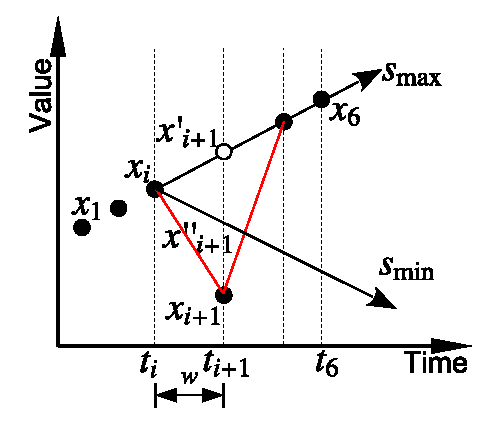
\includegraphics[width=0.6\figwidths]{fig/speed}%\vspace{-1em}
\caption{An example of speed constraints}
\label{fig-speed}
\end{figure}


\paragraph{Application}
Owing to unreliable sensor reading, or erroneous extraction of stock prices, the stream data are often dirty.
Based on speed constraints, Song et al. propose a linear time and constant space cleaning approach for stream data cleaning,  towards local optimum under an efficient \emph{Median Principle}.
The algorithm can avoid changing those originally correct/clean data, i.e. observe the \emph{minimum change principle} in data cleaning.



\subsection{Temporal Constraints}
\label{sect-Temporal-Constraint}

Dechter et al. \cite{DBLP:journals/ai/DechterMP91} introduce \emph{temporal constraint satisfaction problem} (TCSP),
where variables represent time points and temporal information is represented by a set of unary or binary constraints, each specifying a set of permitting intervals.

\paragraph{Notation}
A temporal constraints can be presented by a set of intervals:
$$ \{[\mathit{a}_1, \mathit{b}_1], \dots, [\mathit{a}_n, \mathit{b}_n]\}. $$
According to the different types of the constrains, it represents different meanings:
a unary constraint $\mathit{T}_i$ restricting the domain of variable $\mathit{X}_i$ represents the disjunction
$$(\mathit{a}_1 \leq \mathit{X}_i \leq \mathit{b}_1) \vee \dots \vee (\mathit{a}_n \leq \mathit{X}_i \leq \mathit{b}_n),$$
while a binary constraint $\mathit{T}_{ij}$ constraints the value for distance $\mathit{X}_i - \mathit{X}_j$, which represents the disjunction
$$(\mathit{a}_1 \leq \mathit{X}_i - \mathit{X}_j \leq \mathit{b}_1) \vee \dots \vee (\mathit{a}_n \leq \mathit{X}_i - \mathit{X}_j \leq \mathit{b}_n),$$

A  temporal constraint satisfaction problem involves a set of variables, $\mathit{X}_1, \dots, \mathit{X}_n$,
having continuous domains, and each variable represents a time point.
A special time point $\mathit{X}_0$ represents the beginning of the world, and all times are relative to $\mathit{X}_0$.
Therefore, a unary constraint $\mathit{X}_i$ could be treated as a binary constraint $\mathit{X}_{0i}$.
The solution of the problem is a tuple $\mathit{X} = (\mathit{x}_1, \dots, \mathit{x}_n)$ satisfying all the constraints.

\paragraph{Example}

Figure \ref{fig-temporal-event} presents an example temporal constraint network from  \cite{DBLP:journals/pvldb/SongC016}. 
It denotes the steps (a.k.a. events, denoted by nodes) that are required in every part design process of a train manufacturer. 
The temporal network (abstracted from workflow specifications) specifies the constraints on occurring timestamps of events. 
For instance, the temporal constraint $[1,30]$ from event 1 (\textsf{submit}) to event 3 (\textsf{proofread}) indicates the minimum and maximum restrictions on the distance (delay) of these two events' timestamps. 
That is, event 3 (\textsf{proofread}) should be processed within 30 minutes after event 1 (\textsf{submit}).
%
Multiple intervals may also be declared between two events. 
For instance, $[1,10],[30,40]$ on edge $4\rightarrow5$ denote that event 5 (\textsf{authorize}) can be processed after event 4 (\textsf{examine}) either by the department head in 1-10 minutes or by the division head in 30-40 minutes. 

Consider a corresponding example instance of event trace in Table \ref{table-temporal-event}.
It records one instance of five steps (events) for processing a part design work, including \textsf{submit, normalize, proofread}, etc.
Each event is associated with a timestamp on when this event occurred. 
%
Events 3 and 1 in $t_3$ and $t_1$ satisfy the temporal constraint, since their timestamp distance $09{:}25-09{:}05=20$ is in the range of $[1,30]$.
%
Note that the events are collected from various external sources. 
Imprecise timestamps are prevalent, e.g., {23:53} of event 2 (\textsf{normalize}) in $t_5$, which is delayed until just before midnight owing to latency.
The imprecise timestamps are identified as violations of the temporal constraints, such as events 2 and 1 with timestamp distance $23{:}53-09{:}05=888>30$.

 \begin{table}
 \centering\small
 \caption{An example relation instance of events} 
 \label{table-temporal-event}
% \renewcommand{\arraystretch}{1.5}
 \begin{tabular}{lll}
 \toprule
 & \textsf{event} & \textsf{timestamp}  \\ 
 \midrule 
 $t_1$ & 1 (\textsf{submit})    & 09:05 \\ 
 $t_2$ & 5 (\textsf{authorize}) & 09:54 \\ 
 $t_3$ & 3 (\textsf{proofread}) & 09:25 \\ 
 $t_4$ & 4 (\textsf{examine})   & 09:48 \\ 
 $t_5$ & 2 (\textsf{normalize}) & \textbf{23:53} \\ 
 \bottomrule
 \end{tabular}
 \end{table}

%\Figure[t!](topskip=0pt, botskip=0pt, midskip=0pt)[width=0.8\figwidths]{fig/temporal-event}
%{An example temporal constraint network\label{fig-temporal-event}}

%\Figure[t!](topskip=0pt, botskip=0pt, midskip=0pt)[width=0.8\figwidths]{fig/TCSP_network}
%{A network of binary constraints\label{fig:network_constraint}}

\begin{figure}[t]
\centering
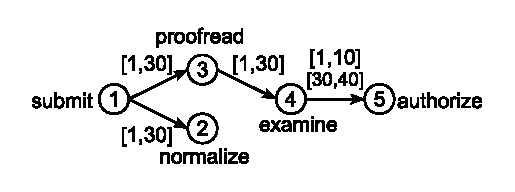
\includegraphics[width=0.8\figwidths]{fig/temporal-event}
\caption{An example temporal constraint network}
\label{fig-temporal-event}
\end{figure}



\paragraph{Application}
Based on temporal constraints, Dechter et al. \cite{DBLP:journals/ai/DechterMP91} present algorithms for performing the following reasoning tasks:
(1) finding all feasible times that a given event can occur;
(2) finding all possible relationships between two given events;
(3) generating one or more scenarios consistent with the information provided.
Song et al. \cite{DBLP:journals/pvldb/SongC016}
utilize the temporal constraints to repair the erroneous timestamps.



\subsection{Summary and Discussion}

To capture the constraints on numerical data, a typical idea is to study the order relationships between numbers, 
such as the order dependencies (ODs) \cite{DBLP:conf/sigmod/DongH82} or denial constraints (DCs) \cite{DBLP:conf/dbpl/BertossiBFL05,DBLP:journals/is/BertossiBFL08} expressed by $<,\leq,>,\geq$.
The specific differences between numerical values, however, are not addressed. 
In this sense, data dependencies with distance metics, such as differential dependencies (DDs) \cite{DBLP:journals/tods/Song011}, can also be employed to state the constraints on distances between numerical values.

For a special type numerical data with temporal information, sequential dependencies (SDs) \cite{DBLP:journals/pvldb/GolabKKSS09} studies both the order of numerical data (e.g., timestamps) as well as the distance. 
Speed constraints \cite{DBLP:conf/sigmod/SongZWY15} extend further by considering the distances on both timestamps and numerical values, known as speeds of value changes.  
Unfortunately, it is not well studied yet on how to discover such meaningful constraints. 

%-------------------------------------------------------------------------
\section{基于统计的清洗方法}
基于统计的清洗算法在数据清洗领域占据重要的位置。此类算法利用从数据 中学习出的模型来进行数据清洗。 

\subsection{贝叶斯模型}
Wang 等人[46] 通过贝叶斯分析建立了一个代价模型,利用该模型对数据中存在的错误进行分析。Bergman 等人[47] 考虑了用户的参与,利 用了用户对于查询结果的反馈信息,对数据进行清洗。  


\subsection{贝叶斯模型}
隐马尔可夫模型是关于时间序列数据的概率模型,描述由一个隐藏的马尔可夫链随机生成的不可观测的状态随机序列,再由各个状态生成一个观测而产生观测随机序列,序列的每一个位置又可以看成是一个时刻,在时间序列数据中隐含的信息通常是指时间。
\subsection{似然估计}
Yakout 等人[33] 提出了基于似然的关系型数据清洗方法。对于待清洗的关系表, 一些带有错误数据的属性被称为灵活属性,这些属性下的数值可以被修改。而其 他的属性则认为包含正确数据,被称为可靠属性。可靠属性和灵活属性之间的关 系可以进行建模,依靠该模型进行灵活属性中数值的清洗。


\subsection{Summary and Discussion}
Mayfield 等人[48] 提出了一个更加复杂的关系依赖网络 (RDN[49]) 模型来对属性之间的概率关系进行建模。RDN 和传统关系依赖(例如贝叶斯网[50])的不同之 处在于 RDN 可以包含环结构。该方法迭代式地对数据集进行清洗,观察每次清洗 之前和之后数据集的概率分布变化。当数据集的概率分布收敛(即清洗前后差别 小于一个给定阈值)时,清洗过程中止。该方法很大程度依赖 RDN 的选择,如果 待清洗时间序列无法给出合理的 RDN,那么该方法清洗效果无法得到保证。Zhou 等人[51] 提出了用 GPU 来对高斯模型的学习进行加速的方法。该文章认为在数据 量过大的情况下,没有必要使用全部的数据用来学习模型,相反,利用 k 近邻[52] 的思想,只需要利用距离(利用 DTW[53] 算法计算距离)待预测数据最近的 k 条,数据即可。除此之外,该文章还提供了自动调参的方法。

%-------------------------------------------------------------------------
\section{时间序列异常检测算法}
Hellerstein[56] 调研了清洗大型数据库中数值属性错误的方法。在该调研中,时间序列数据被视作一种特殊情况。 Gupta 等人[10] 对时序相关数据的异常检测方法进行了调研:对一个给定的时间序列,可能有两大类异常的情况,即单点异常和子序列异常(连续异常)。对于单点异常,最常用的做法是利用预测模型来进行检测。即比较所建立模 型对于每个数据点的预测值和观测值,如果这两个值之间差值大于一定阈值,则 认为该观测值为异常值。具体地,Basu 等人[57] 以时间戳 t 为中心点,选取时间戳 为 t-k 到 t+k 的所有数据点,这些数据点的中位数被认为是时间戳为 t 的数据点的 预测值。Hill 等人[58] 则首先将数据点聚类,并取聚类的平均值作为该点的预测值。 自回归 (AR) 模型和带有外部依赖的自回归 (ARX) 实际上被广泛用于多种领域的异 常检测,例如经济学领域,社会调查[2,3] 等等。ARX 模型能够利用人工标注的信息, 因此在数据清洗时会比 AR 模型要更加准确一些。ARIMA 模型[21] 代表着一类时间 序列模型,由前文中提到的 AR 过程和 MA 过程两大类别组成。其中的 I 代表差 分阶数。故该模型可以用于非平稳时间序列的建模。亦可以用于非平稳时间序列 的数据清洗。 

\par 对于子序列异常,不同的研究有着不同的定义。Keogh 等人[63] 认为,所谓子 序列异常即某个子序列与和它最近的非重叠匹配具有最大距离。在这个定义下,最 简单的计算方法就是计算每一个长度为 n 的子序列与其他子序列之间的距离。当然这样做时间开销会很大,为此 Keogh 等人[64] 提出了将候选子序列进行重排序的 启发式算法,Wei 等人[65] 提出了利用局部敏感哈希值的加速算法等等。在计算距 离时,通常使用欧氏距离,而 Keogh[66] 又进一步提出了利用基于压缩的相似度度 量 (CDM) 来作为距离函数的方法。除此之外,Yankov 等人[67] 还提出了解决存储 于硬盘上的大规模时间序列子序列异常检测的方案。 接下来,我们将一些常用的异常检测算法展开叙述。

\subsection{时间窗口下基于相似度匹配的异常检测 }
如图 2.8[35]所示,与上一小节相比,这一小节的数据被分成多个相互带有重 叠的子序列即窗口。先计算每个窗口异常分数,然后根据各个窗口的异常分数 (AS)计算整个测试序列的异常分数(AS),与将整个时间序列直接输出为异 常值相比,基于窗口的技术能够更好的定位异常。基于这种技术的方法有两大类, 一类是通过维护一个正常数据库[36-37],设定窗口的大小,再将测试序列与正常数 据库中的序列相匹配,如果数据库中没有测试序列也可以对其不匹配度进行计 算,进而判断是否异常;另一类是构建异常的数据库[38-39],然后将测试序列与该 数据库匹配,进而检测异常。 


\subsection{基于密度的时序数据异常检测}
基于密度的异常数据可以理解为错误! 未找到引用源。:给定一种密度计算方法,可以为每一个数据点计算其周围数据密度。若某一数据点的数据密度与其相邻数据点(neighbors)数据密度差异显著,则称该点为异常数据。目前在时序数据中局部异常因子算法及其各个变种方法应用较为广泛,接下来我们首先介绍下基础的LOF[41]算法,然后介绍用于时序数据异常检测的增量式LOF算法[42]。


\subsection{Summary and Discussion }

在时间序列异常检测算法中,一些由于采集误差或者错读、误读等原因造成的异常数据往往被丢弃,使得这些数据的价值没有被充分利用。有一些研究利用时间序列异常检测算法,先对数据进行检测,对检测为异常的数据在结合其他技术进行修复而不是丢弃,这类技术使得原来会被丢弃的技术可以再次被使用,具有很好的应用前景。


%-------------------------------------------------------------------------
\section{Tools and Evaluation criterion}

\subsection{Tools}
(1)Rekatsinas 等人[54] 提出了 HoloClean 数据清洗框架,该清洗框架包含异常检 测、概率编辑和数据清洗三个主要步骤。支持多源的输入,如完整性约束,外源数 据库信息以及输入数据集的概率分布。HoloClean 基于以上的输入,会学习出统一 的概率图模型,然后根据概率分布情况选择最终的数据清洗方案。 
\par (2)例如 Williams 等 人[61] 设计的 Tiresias 系统能够保存正常数据历史画像和方差向量。该历史画像是 历史数据平滑后的时间序列。任何新读入系统的数据点会被用来和之前两个相比 较,并计算出一个代表其异常程度的数值。
\par(3)ASAP

\subsection{Evaluation criterion}
\par(1)错误数据和正确数据间的错误距离 
\par (2)错 误数据和清洗结果间的修复距离 
\par(3)清洗结果和正确数据间的 RMS 误差[68
使用 RMS 误差[68] 来评估清洗算法的效果。令 xtruth 表示时间序列的真 实值组成的序列,xdirty 表示加入了错误以后的观测值组成的序列,xrepair 表示清洗 后的修复值组成的序列。用上述符号表示 RMS 误差[68],有 
\par (4)对于错误数据的清洗准确度[27]
\par(5)Dasu 等人[55] 提 出了统计失真方法来评测清洗方法的质量。该方法直接观察数据集中的数值分布,依据不同清洗方法带来的分布的变化评测其质量。

%-------------------------------------------------------------------------
\section{Conclusion and Future Directions}

\subsection{Conclusion}

随着科技的进步,人们逐渐意识到了数据中蕴含的价值。而传输和存储成本 的降低,更让可以利用的数据达到了新的数量级。各个企业期望从这些数据中得 到具有价值的知识,数据分析在金融、医疗、自然科学、工业领域中也起到了越来 越重要的作用。而时间序列数据作为重要的数据类型,广泛出现于工业制造业之中。例如风电企业中会采集并分析位于风力发电机各处的传感器采集的数据,判 断风机是否处于正常状态;物流车运维企业也希望通过分析车载 GPS 信息来优化 车队的路线管理。然而由于外界环境干扰,传感器自身精度等问题,时间序列数据中往往含有很多的错误。这些错误会干扰后续的数据分析,造成不可预估的影响。 


\subsection{Conclusion}
正如前文所言,时间序列数据在工业领域中起到了越来越重要的作用,互联 网与大数据环境下的制造设备所产生的数据含有十分丰富的价值。时间序列数据 清洗技术为这些价值的发掘提供了非常重要的技术支持。时间序列数据清洗方面含有大量的难点,大数据领域技术也在快速发展,本文认为有很多方面的工作值得进一步探 索,具体如下。 

\par 时间序列数据错误类型图鉴。 截至目前,数据科学家们对传统的关系型数据 库中出现的错误已经有了十分详尽的分析。然而对于时间序列数据错误类型的分 析还有着很多不足之处。例如本文将时间序列中的错误类型大致分为三种,即单 点大错误,单点小错误和连续错误。实际上,在连续错误中,也有非常多的细致的 错误类型,例如文中之前提到过的整体平移型和革新型错误。如何去系统理论地 分析这些错误类型,形成时间序列数据错误类型图鉴,是十分重要的。明确的类 型有助于针对性的清洗算法开发,从而解决当前领域中存在的“GIGO(Garbage in, garbage out. 即错误数据进入,错误结果输出)”的问题。 

\par 时间序列清洗算法设计。 本文各章综述了一些时间序列错误清洗算法,但还可以进行更深入的优化。1)在考虑速度约束时,单纯地使用最小修改原则作为目 标可能并不能使清洗结果达到最优,反而会造成所谓的边界修复结果。可以考虑 放宽目标限制。另外,除了速度约束之外,也可以考虑数据点间的加速度等时序 数据特征,来辅助清洗;2)在考虑最大似然时,单纯地使用连续两点间的速度变 化的概率可能并不准确,如果相邻两点间的时间间隔较大,那么需要考虑时间产生的影响,例如将速度变化变为加速度。除此之外,能否进一步降低精确算法的 时间复杂度,以期得到更好的实际应用效果也是需要思考的;3)在考虑利用标注 信息时,基于的是带有外生变量的自回归模型,但是该模型有着明显的方向性。能 否将一定时间读入的时间序列数据缓存下来,然后在这些数据上从时间顺序的正 序和倒序两方面进行建模和清洗,有可能得到更好的清洗效果。除此之外,本文 提出的方法都是针对于单一维度的时间序列的(即便是 GPS 信号有着两个维度信 息,但是在清洗时是每个维度单独清洗的)。要想进一步提高算法的实用性,考虑 多维时间序列的清洗势在必行。 

\par 时间序列清洗工具实现。除了提供核心的时间序列清洗算法之外,构建时间 序列清洗工具也十分重要。目前工业界主流的数据清洗工具仍然是针对关系型数 据库的,而这些工具在时间序列数据的处理上效果并不理想。如何利用飞速发展的大数据技术实现时间序列清洗工具,并应用于工业领域等真实场景,是下一个 阶段的重点工作。 

\par 时间序列异常检测算法设计。在面对真实应用场景时可看到,如何对收集到 的时间序列进行高效的异常检测同样十分重要。在很多工业场景中,很难判断错 误值和真实值之间的差别,因此需要针对性地设计可以应用于工业场景的时间序 列异常检测算法。另外,如何在先验知识较弱的情况下进行异常检测以及进一步 的清洗和分析,也需要进行进一步的研究。

\par 特定应用场景下数据清洗算法的设计。随着各类技术在产业界的落地应用,业务场景变得越来越细化,不同的业务场景下对清洗算法的要求有不同的侧重点,例如:区块链网络中存储的数据一般为结构化的数据,随着区块链技术的发展,区块链网络上数据清洗算法的设计也显得尤为重要。





%=========================================================================
\bibliographystyle{abbrv}
\bibliography{timeseries}

\end{document}
